\chapter{Study Methodology}
\label{Methodology}

A tradeoff was made and the study was conducted in two phases in order to simultaneously gather more ecologically valid results as well maximize the amount of data collected. The first phase provided insight into participants' typical habits while the second gave more of an indication of their reasoning. The two phases correspond to our two areas of interest for the study: warning message adherence and captivating aspects of messages. An eye tracker was used for both phases of the study to determine where on the warning messages participants spent their time looking.

In short, participants were first exposed to one warning without any prior knowledge of the study. After learning the true purpose, we showed them all combinations of warning severity (low, medium, high, and control) and type (SSL, malware, phishing, and unwanted software) in a random order. We presented a two-question on-screen questionnaire after each message to measure risk perception and allow participants to explain their thought processes.

\section{Phase 1}
Participants did not initially know the true purpose of the study. In the first phase, they were told that we were investigating browsing habits and that they would be interacting with, reacting to, and giving feedback on various web pages. After calibrating the eye tracker, we pretended to have forgotten to show participants a particular form and asked to email it to them (for simplicity). It was mentioned that this was not mandatory, and an option was given to print the form instead if ``something went wrong'' or the participant felt uncomfortable logging in on a computer other than their own.

Upon navigating the web browser to the email login page, a warning message was triggered. Severity and type for this message was changed between participants. The software used to trigger the warning (detailed in section \ref{Methodology-Software}) noted whether or not participants ignored the message and tried to continue past to their email inbox as well as how long they spent making a decision. We then informed them of the true purpose of the study and clarified that there was no real threat and no data or information was at risk.

The goal of this phase is to obtain plausibly realistic results. This is encouraged in two ways. First, we suspect that participants will be more reluctant to ignore warning messages when their own personal information is supposedly at stake (e.g., their email login credentials and email messages themselves). Secondly, by being uninformed as to the study's true purpose, some bias will be removed. The behaviour will thereby more closely match that which would be observed in a non-laboratory environment.

\section{Phase 2}
The second phase involved participants reacting to various warning messages that they were presented with (either by clicking the ``go back'' or ``ignore'' button). The goal here is to obtain more data with regards to warning adherence, as well as to delve deeper into what makes a given warning worth paying attention to for participants. The tradeoff is that the data collected in this phase is less ecologically valid. Each participant was shown warnings of all types and severity levels mentioned above, with the ordering randomized.

In both phases of the study, the following questionnaire was displayed after each warning:

\begin{enumerate}
	\item How do you rate the severity of the warning message you just saw?
	\begin{center}
		\begin{tabular}{ccccc}
			Very low & Low & Medium & High & Very high\\
		\end{tabular}
	\end{center}
	\item Please explain the reason(s) for your answer to question 1 and choice to visit/not visit the fictional page.
\end{enumerate}


\section{Recruitment of Participants}
Participants for the study were recruited through social media, posters, and snowballing. An invitation to participate was posted on the researcher's Facebook page as well as a group page for individuals interested participating in studies at Carleton University. Posters using the same text as the social media invitation were also placed in typically busy locations around the Carleton University campus. In both of these cases, the study was described as being about web browsing habits so as to not compromise the deceptive aspect of the first phase. After completing the study, participants were encouraged to mention it to others (without divulging its true purpose and the deception employed in the first phase).

20 participants aged 18-57 took part in the study. All indicated on the demographic questionnaire that they browsed the web multiple times per day (10 on a mobile device and 10 on a PC). 10 participants were male, 9 were female, and one identified as genderfluid. Additionally, 7 of the participants indicated that they had a computer science background or had programmed before.


\section{Ethics}
Ethics approval for the study was obtained through Carleton University's Research Ethics Board prior to the recruitment of participants and the start of the study. Participants were each compensated \$10 CAD, regardless of whether or not they withdrew from the study.


\section{Software}
\label{Methodology-Software}
We developed a browser extension for Mozilla Firefox to display the different warning messages\footnote{See \url{http://github.com/mwpenny/warning-sim} for the source code.}. This approach was chosen so that messages could be shown in as realistic an environment as possible (i.e., within the browser itself, as opposed to static images). It also enables interactivity (e.g., the ``more information'' button can be clicked by curious users to reveal additional text describing the warning).

\begin{figure}[th]
	\centering
	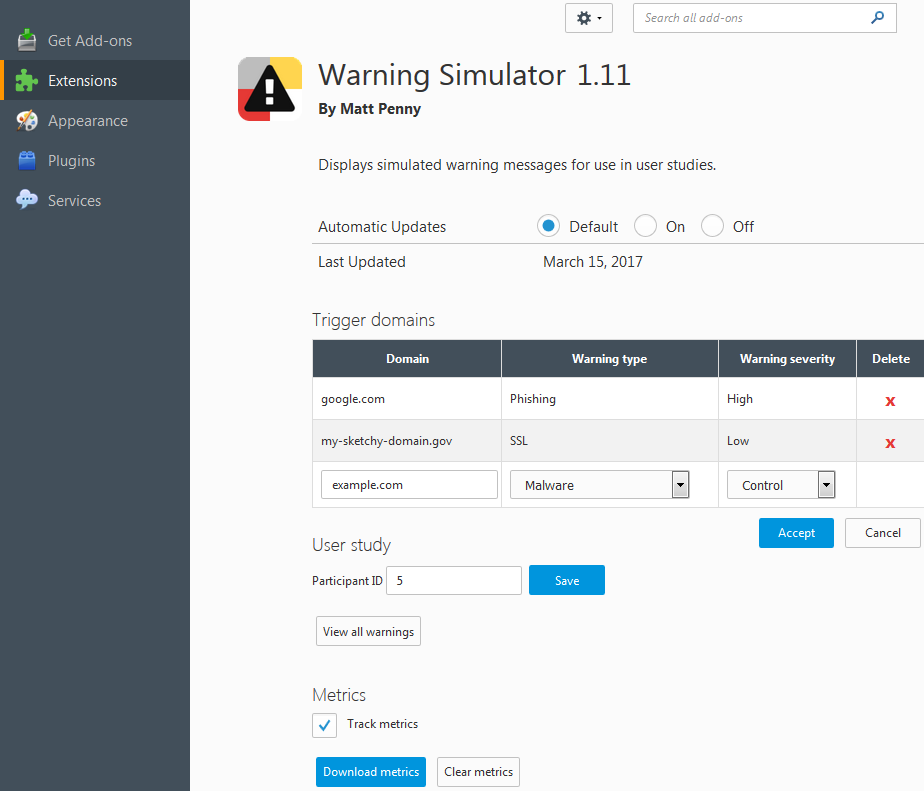
\includegraphics[width=0.925\textwidth]{Figures/Warning-Sim}
	\decoRule
	\caption[Warning simulator control panel]{The browser extension's configuration page. Experimenters can specify trigger domains, view all messages in a random order, and more.}
	\label{fig:Warning-Sim}
\end{figure}

Internal Firefox styling was also used to give the messages a look and feel similar to other ones users might have previously seen in the browser, adding to their authenticity. All of these factors result in a more realistic and authentic experience. Additionally, using web technologies to design the messages permitted quick and easy changes.

The extension allows an experimenter to specify a list of trigger domains for which warning messages should be displayed upon visiting (illustrated in figure \ref{fig:Warning-Sim}). For each domain, the warning type can be specified along with its severity. Alternately, a control message can be shown. This is useful for facilitating phase 1 of the study, in which unsuspecting participants are shown a warning message upon browsing to their email login page. There is also the ability to view all of the study's warning messages in a random order, one after the other -- enabling phase 2 of the study to be easily conducted.

The most obvious benefit of the browser extension is ease of data collection. Code was included to track which buttons were clicked and how much time was spent viewing a given warning before a decision was made, for example. The questionnaire mentioned above is also displayed after a warning's ``go back'' or ``ignore'' button is selected, easing the gathering of these responses for the two questions asked repeatedly throughout the study. All of this data is taggable with a configurable, anonymous participant ID and can be exported as a CSV spreadsheet.

Valuable data is also collected by the eye tracker, which records where participants look on screen and for how long. Visualizations such as heat maps and eye gaze trails can be superimposed over captured screen recordings. This information can be used to infer which aspects of the messages are most captivating to users.
